% Fig. 1 (fig:overview). Compile standalone with pdflatex and copy the PDF to figs/fig_llm_position.pdf.
\documentclass[tikz,border=1.5pt]{standalone}
\usepackage[T1]{fontenc}
\usepackage{helvet}
\usepackage{sansmath}
\renewcommand{\familydefault}{\sfdefault}
\usetikzlibrary{arrows.meta,shapes.symbols,shapes.geometric,calc}
\definecolor{ink}{HTML}{1A1A1A}
\definecolor{mute}{HTML}{6B6B6B}
\definecolor{panel}{HTML}{F4F4F4}
\definecolor{neuF}{HTML}{E6E6E6}
\definecolor{neuS}{HTML}{8A8A8A}
\definecolor{llmF}{HTML}{CDEBEA}\definecolor{llmS}{HTML}{2A8C90}
\definecolor{codeF}{HTML}{EAF6F5}
\definecolor{arr}{HTML}{404040}
\begin{document}
\sansmath
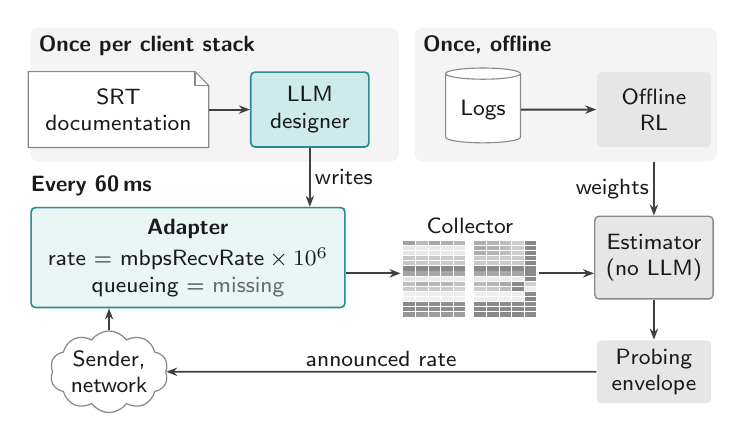
\begin{tikzpicture}[x=1cm,y=1cm, font=\footnotesize, text=ink,
  flow/.style={-{Stealth[length=4pt,width=3pt]}, draw=arr, line width=0.7pt},
  gtitle/.style={anchor=north west, inner sep=0pt, font=\footnotesize\bfseries},
  box/.style={align=center, inner xsep=4pt, inner ysep=2pt, rounded corners=1.5pt},
]
\fill[panel, rounded corners=3pt] (0,3.42) rectangle (4.68,5.12);
\node[gtitle] at (0.1,5.02) {Once per client stack};
\node[align=center, inner xsep=6pt, inner ysep=4pt, minimum width=1.9cm, minimum height=0.95cm] (doc) at (1.12,4.08) {\phantom{SRT}\\\phantom{documentation}};
\filldraw[fill=white, draw=neuS, line width=0.4pt] (doc.south west) -- (doc.south east) -- ([yshift=-5pt]doc.north east) -- ([xshift=-5pt]doc.north east) -- (doc.north west) -- cycle;
\draw[neuS, line width=0.4pt] ([xshift=-5pt]doc.north east) -- ([xshift=-5pt,yshift=-5pt]doc.north east) -- ([yshift=-5pt]doc.north east);
\node[align=center] at (doc.center) {SRT\\documentation};
\node[box, fill=llmF, draw=llmS, line width=0.6pt, minimum width=1.5cm, minimum height=0.95cm] (llm) at (3.55,4.08) {LLM\\designer};
\draw[flow] (doc.east) -- (llm.west);
\fill[panel, rounded corners=3pt] (4.88,3.42) rectangle (8.72,5.12);
\node[gtitle] at (4.98,5.02) {Once, offline};
\node[cylinder, shape border rotate=90, aspect=0.22, draw=neuS, fill=white, line width=0.4pt, minimum width=0.95cm, minimum height=0.95cm, align=center, inner sep=1pt] (logs) at (5.75,4.08) {Logs};
\node[box, fill=neuF, minimum width=1.45cm, minimum height=0.95cm] (off) at (7.92,4.08) {Offline\\RL};
\draw[flow] (logs.east) -- (off.west);
\node[gtitle] at (0.0,3.24) {Every 60\,ms};
\node[anchor=west, fill=codeF, draw=llmS, line width=0.6pt, rounded corners=1.5pt, align=center, inner xsep=6pt, inner ysep=4pt, minimum height=1.2cm] (ad) at (0.0,2.2) {%
  \textbf{Adapter}\\[2pt]
  rate = mbpsRecvRate${}\times10^{6}$\\
  queueing = \textcolor{mute}{missing}};
\draw[flow] (llm.south) -- node[right=1.5pt, inner sep=0pt] {writes} (llm.south|-ad.north);
\node[box, fill=neuF, draw=neuS, line width=0.5pt, minimum width=1.45cm, minimum height=1.05cm] (est) at (7.92,2.2) {Estimator\\(no LLM)};
\node[box, fill=neuF, minimum width=1.45cm, minimum height=0.8cm] (env) at (7.92,0.75) {Probing\\envelope};
\coordinate (gx) at ($(ad.east)!0.5!(est.west)+(-0.85,0)$);
\begin{scope}[shift={($(gx|-0,2.42)+(-8.0,-2.06)$)}]% Generated by scripts/paper/make_fig1_collector_grid_v1.py --palette greys --lighten 0.4; do not edit. Data: the observation 60.05 s after shaping starts in obs_arm_llm4bandpp_x__hd_c2__d0__r1__vjohnny.jsonl.gz.
\fill[fill={rgb,255:red,161;green,161;blue,161}] (8.0060,2.0540) rectangle (8.1540,2.0010);
\fill[fill={rgb,255:red,185;green,185;blue,185}] (8.1660,2.0540) rectangle (8.3140,2.0010);
\fill[fill={rgb,255:red,167;green,167;blue,167}] (8.3260,2.0540) rectangle (8.4740,2.0010);
\fill[fill={rgb,255:red,175;green,175;blue,175}] (8.4860,2.0540) rectangle (8.6340,2.0010);
\fill[fill={rgb,255:red,182;green,182;blue,182}] (8.6460,2.0540) rectangle (8.7940,2.0010);
\fill[fill={rgb,255:red,172;green,172;blue,172}] (8.9060,2.0540) rectangle (9.0540,2.0010);
\fill[fill={rgb,255:red,179;green,179;blue,179}] (9.0660,2.0540) rectangle (9.2140,2.0010);
\fill[fill={rgb,255:red,190;green,190;blue,190}] (9.2260,2.0540) rectangle (9.3740,2.0010);
\fill[fill={rgb,255:red,204;green,204;blue,204}] (9.3860,2.0540) rectangle (9.5340,2.0010);
\fill[fill={rgb,255:red,137;green,137;blue,137}] (9.5460,2.0540) rectangle (9.6940,2.0010);
\fill[fill={rgb,255:red,231;green,231;blue,231}] (8.0060,1.9890) rectangle (8.1540,1.9360);
\fill[fill={rgb,255:red,233;green,233;blue,233}] (8.1660,1.9890) rectangle (8.3140,1.9360);
\fill[fill={rgb,255:red,231;green,231;blue,231}] (8.3260,1.9890) rectangle (8.4740,1.9360);
\fill[fill={rgb,255:red,232;green,232;blue,232}] (8.4860,1.9890) rectangle (8.6340,1.9360);
\fill[fill={rgb,255:red,233;green,233;blue,233}] (8.6460,1.9890) rectangle (8.7940,1.9360);
\fill[fill={rgb,255:red,170;green,170;blue,170}] (8.9060,1.9890) rectangle (9.0540,1.9360);
\fill[fill={rgb,255:red,176;green,176;blue,176}] (9.0660,1.9890) rectangle (9.2140,1.9360);
\fill[fill={rgb,255:red,187;green,187;blue,187}] (9.2260,1.9890) rectangle (9.3740,1.9360);
\fill[fill={rgb,255:red,203;green,203;blue,203}] (9.3860,1.9890) rectangle (9.5340,1.9360);
\fill[fill={rgb,255:red,137;green,137;blue,137}] (9.5460,1.9890) rectangle (9.6940,1.9360);
\fill[fill={rgb,255:red,230;green,230;blue,230}] (8.0060,1.9240) rectangle (8.1540,1.8710);
\fill[fill={rgb,255:red,233;green,233;blue,233}] (8.1660,1.9240) rectangle (8.3140,1.8710);
\fill[fill={rgb,255:red,231;green,231;blue,231}] (8.3260,1.9240) rectangle (8.4740,1.8710);
\fill[fill={rgb,255:red,232;green,232;blue,232}] (8.4860,1.9240) rectangle (8.6340,1.8710);
\fill[fill={rgb,255:red,233;green,233;blue,233}] (8.6460,1.9240) rectangle (8.7940,1.8710);
\fill[fill={rgb,255:red,172;green,172;blue,172}] (8.9060,1.9240) rectangle (9.0540,1.8710);
\fill[fill={rgb,255:red,179;green,179;blue,179}] (9.0660,1.9240) rectangle (9.2140,1.8710);
\fill[fill={rgb,255:red,190;green,190;blue,190}] (9.2260,1.9240) rectangle (9.3740,1.8710);
\fill[fill={rgb,255:red,204;green,204;blue,204}] (9.3860,1.9240) rectangle (9.5340,1.8710);
\fill[fill={rgb,255:red,137;green,137;blue,137}] (9.5460,1.9240) rectangle (9.6940,1.8710);
\fill[fill={rgb,255:red,198;green,198;blue,198}] (8.0060,1.8590) rectangle (8.1540,1.8060);
\fill[fill={rgb,255:red,202;green,202;blue,202}] (8.1660,1.8590) rectangle (8.3140,1.8060);
\fill[fill={rgb,255:red,202;green,202;blue,202}] (8.3260,1.8590) rectangle (8.4740,1.8060);
\fill[fill={rgb,255:red,202;green,202;blue,202}] (8.4860,1.8590) rectangle (8.6340,1.8060);
\fill[fill={rgb,255:red,201;green,201;blue,201}] (8.6460,1.8590) rectangle (8.7940,1.8060);
\fill[fill={rgb,255:red,201;green,201;blue,201}] (8.9060,1.8590) rectangle (9.0540,1.8060);
\fill[fill={rgb,255:red,202;green,202;blue,202}] (9.0660,1.8590) rectangle (9.2140,1.8060);
\fill[fill={rgb,255:red,202;green,202;blue,202}] (9.2260,1.8590) rectangle (9.3740,1.8060);
\fill[fill={rgb,255:red,202;green,202;blue,202}] (9.3860,1.8590) rectangle (9.5340,1.8060);
\fill[fill={rgb,255:red,137;green,137;blue,137}] (9.5460,1.8590) rectangle (9.6940,1.8060);
\fill[fill={rgb,255:red,198;green,198;blue,198}] (8.0060,1.7940) rectangle (8.1540,1.7410);
\fill[fill={rgb,255:red,202;green,202;blue,202}] (8.1660,1.7940) rectangle (8.3140,1.7410);
\fill[fill={rgb,255:red,202;green,202;blue,202}] (8.3260,1.7940) rectangle (8.4740,1.7410);
\fill[fill={rgb,255:red,202;green,202;blue,202}] (8.4860,1.7940) rectangle (8.6340,1.7410);
\fill[fill={rgb,255:red,201;green,201;blue,201}] (8.6460,1.7940) rectangle (8.7940,1.7410);
\fill[fill={rgb,255:red,201;green,201;blue,201}] (8.9060,1.7940) rectangle (9.0540,1.7410);
\fill[fill={rgb,255:red,202;green,202;blue,202}] (9.0660,1.7940) rectangle (9.2140,1.7410);
\fill[fill={rgb,255:red,202;green,202;blue,202}] (9.2260,1.7940) rectangle (9.3740,1.7410);
\fill[fill={rgb,255:red,202;green,202;blue,202}] (9.3860,1.7940) rectangle (9.5340,1.7410);
\fill[fill={rgb,255:red,137;green,137;blue,137}] (9.5460,1.7940) rectangle (9.6940,1.7410);
\fill[fill={rgb,255:red,137;green,137;blue,137}] (8.0060,1.7290) rectangle (8.1540,1.6760);
\fill[fill={rgb,255:red,137;green,137;blue,137}] (8.1660,1.7290) rectangle (8.3140,1.6760);
\fill[fill={rgb,255:red,137;green,137;blue,137}] (8.3260,1.7290) rectangle (8.4740,1.6760);
\fill[fill={rgb,255:red,137;green,137;blue,137}] (8.4860,1.7290) rectangle (8.6340,1.6760);
\fill[fill={rgb,255:red,137;green,137;blue,137}] (8.6460,1.7290) rectangle (8.7940,1.6760);
\fill[fill={rgb,255:red,137;green,137;blue,137}] (8.9060,1.7290) rectangle (9.0540,1.6760);
\fill[fill={rgb,255:red,137;green,137;blue,137}] (9.0660,1.7290) rectangle (9.2140,1.6760);
\fill[fill={rgb,255:red,137;green,137;blue,137}] (9.2260,1.7290) rectangle (9.3740,1.6760);
\fill[fill={rgb,255:red,137;green,137;blue,137}] (9.3860,1.7290) rectangle (9.5340,1.6760);
\fill[fill={rgb,255:red,137;green,137;blue,137}] (9.5460,1.7290) rectangle (9.6940,1.6760);
\fill[fill={rgb,255:red,164;green,164;blue,164}] (8.0060,1.6640) rectangle (8.1540,1.6110);
\fill[fill={rgb,255:red,166;green,166;blue,166}] (8.1660,1.6640) rectangle (8.3140,1.6110);
\fill[fill={rgb,255:red,166;green,166;blue,166}] (8.3260,1.6640) rectangle (8.4740,1.6110);
\fill[fill={rgb,255:red,166;green,166;blue,166}] (8.4860,1.6640) rectangle (8.6340,1.6110);
\fill[fill={rgb,255:red,166;green,166;blue,166}] (8.6460,1.6640) rectangle (8.7940,1.6110);
\fill[fill={rgb,255:red,165;green,165;blue,165}] (8.9060,1.6640) rectangle (9.0540,1.6110);
\fill[fill={rgb,255:red,166;green,166;blue,166}] (9.0660,1.6640) rectangle (9.2140,1.6110);
\fill[fill={rgb,255:red,166;green,166;blue,166}] (9.2260,1.6640) rectangle (9.3740,1.6110);
\fill[fill={rgb,255:red,166;green,166;blue,166}] (9.3860,1.6640) rectangle (9.5340,1.6110);
\fill[fill={rgb,255:red,137;green,137;blue,137}] (9.5460,1.6640) rectangle (9.6940,1.6110);
\fill[fill={rgb,255:red,229;green,229;blue,229}] (8.0060,1.5990) rectangle (8.1540,1.5460);
\fill[fill={rgb,255:red,233;green,233;blue,233}] (8.1660,1.5990) rectangle (8.3140,1.5460);
\fill[fill={rgb,255:red,234;green,234;blue,234}] (8.3260,1.5990) rectangle (8.4740,1.5460);
\fill[fill={rgb,255:red,234;green,234;blue,234}] (8.4860,1.5990) rectangle (8.6340,1.5460);
\fill[fill={rgb,255:red,234;green,234;blue,234}] (8.6460,1.5990) rectangle (8.7940,1.5460);
\fill[fill={rgb,255:red,233;green,233;blue,233}] (8.9060,1.5990) rectangle (9.0540,1.5460);
\fill[fill={rgb,255:red,234;green,234;blue,234}] (9.0660,1.5990) rectangle (9.2140,1.5460);
\fill[fill={rgb,255:red,235;green,235;blue,235}] (9.2260,1.5990) rectangle (9.3740,1.5460);
\fill[fill={rgb,255:red,233;green,233;blue,233}] (9.3860,1.5990) rectangle (9.5340,1.5460);
\fill[fill={rgb,255:red,137;green,137;blue,137}] (9.5460,1.5990) rectangle (9.6940,1.5460);
\fill[fill={rgb,255:red,190;green,190;blue,190}] (8.0060,1.5340) rectangle (8.1540,1.4810);
\fill[fill={rgb,255:red,178;green,178;blue,178}] (8.1660,1.5340) rectangle (8.3140,1.4810);
\fill[fill={rgb,255:red,183;green,183;blue,183}] (8.3260,1.5340) rectangle (8.4740,1.4810);
\fill[fill={rgb,255:red,181;green,181;blue,181}] (8.4860,1.5340) rectangle (8.6340,1.4810);
\fill[fill={rgb,255:red,193;green,193;blue,193}] (8.6460,1.5340) rectangle (8.7940,1.4810);
\fill[fill={rgb,255:red,187;green,187;blue,187}] (8.9060,1.5340) rectangle (9.0540,1.4810);
\fill[fill={rgb,255:red,182;green,182;blue,182}] (9.0660,1.5340) rectangle (9.2140,1.4810);
\fill[fill={rgb,255:red,167;green,167;blue,167}] (9.2260,1.5340) rectangle (9.3740,1.4810);
\fill[fill={rgb,255:red,137;green,137;blue,137}] (9.3860,1.5340) rectangle (9.5340,1.4810);
\fill[fill={rgb,255:red,206;green,206;blue,206}] (9.5460,1.5340) rectangle (9.6940,1.4810);
\fill[fill={rgb,255:red,203;green,203;blue,203}] (8.0060,1.4690) rectangle (8.1540,1.4160);
\fill[fill={rgb,255:red,200;green,200;blue,200}] (8.1660,1.4690) rectangle (8.3140,1.4160);
\fill[fill={rgb,255:red,202;green,202;blue,202}] (8.3260,1.4690) rectangle (8.4740,1.4160);
\fill[fill={rgb,255:red,202;green,202;blue,202}] (8.4860,1.4690) rectangle (8.6340,1.4160);
\fill[fill={rgb,255:red,210;green,210;blue,210}] (8.6460,1.4690) rectangle (8.7940,1.4160);
\fill[fill={rgb,255:red,206;green,206;blue,206}] (8.9060,1.4690) rectangle (9.0540,1.4160);
\fill[fill={rgb,255:red,202;green,202;blue,202}] (9.0660,1.4690) rectangle (9.2140,1.4160);
\fill[fill={rgb,255:red,188;green,188;blue,188}] (9.2260,1.4690) rectangle (9.3740,1.4160);
\fill[fill={rgb,255:red,137;green,137;blue,137}] (9.3860,1.4690) rectangle (9.5340,1.4160);
\fill[fill={rgb,255:red,235;green,235;blue,235}] (9.5460,1.4690) rectangle (9.6940,1.4160);
\fill[fill={rgb,255:red,238;green,238;blue,238}] (8.0060,1.4040) rectangle (8.1540,1.3510);
\fill[fill={rgb,255:red,238;green,238;blue,238}] (8.1660,1.4040) rectangle (8.3140,1.3510);
\fill[fill={rgb,255:red,238;green,238;blue,238}] (8.3260,1.4040) rectangle (8.4740,1.3510);
\fill[fill={rgb,255:red,238;green,238;blue,238}] (8.4860,1.4040) rectangle (8.6340,1.3510);
\fill[fill={rgb,255:red,238;green,238;blue,238}] (8.6460,1.4040) rectangle (8.7940,1.3510);
\fill[fill={rgb,255:red,238;green,238;blue,238}] (8.9060,1.4040) rectangle (9.0540,1.3510);
\fill[fill={rgb,255:red,238;green,238;blue,238}] (9.0660,1.4040) rectangle (9.2140,1.3510);
\fill[fill={rgb,255:red,238;green,238;blue,238}] (9.2260,1.4040) rectangle (9.3740,1.3510);
\fill[fill={rgb,255:red,238;green,238;blue,238}] (9.3860,1.4040) rectangle (9.5340,1.3510);
\fill[fill={rgb,255:red,137;green,137;blue,137}] (9.5460,1.4040) rectangle (9.6940,1.3510);
\fill[fill={rgb,255:red,238;green,238;blue,238}] (8.0060,1.3390) rectangle (8.1540,1.2860);
\fill[fill={rgb,255:red,238;green,238;blue,238}] (8.1660,1.3390) rectangle (8.3140,1.2860);
\fill[fill={rgb,255:red,238;green,238;blue,238}] (8.3260,1.3390) rectangle (8.4740,1.2860);
\fill[fill={rgb,255:red,238;green,238;blue,238}] (8.4860,1.3390) rectangle (8.6340,1.2860);
\fill[fill={rgb,255:red,238;green,238;blue,238}] (8.6460,1.3390) rectangle (8.7940,1.2860);
\fill[fill={rgb,255:red,238;green,238;blue,238}] (8.9060,1.3390) rectangle (9.0540,1.2860);
\fill[fill={rgb,255:red,238;green,238;blue,238}] (9.0660,1.3390) rectangle (9.2140,1.2860);
\fill[fill={rgb,255:red,238;green,238;blue,238}] (9.2260,1.3390) rectangle (9.3740,1.2860);
\fill[fill={rgb,255:red,238;green,238;blue,238}] (9.3860,1.3390) rectangle (9.5340,1.2860);
\fill[fill={rgb,255:red,137;green,137;blue,137}] (9.5460,1.3390) rectangle (9.6940,1.2860);
\fill[fill={rgb,255:red,137;green,137;blue,137}] (8.0060,1.2740) rectangle (8.1540,1.2210);
\fill[fill={rgb,255:red,143;green,143;blue,143}] (8.1660,1.2740) rectangle (8.3140,1.2210);
\fill[fill={rgb,255:red,141;green,141;blue,141}] (8.3260,1.2740) rectangle (8.4740,1.2210);
\fill[fill={rgb,255:red,142;green,142;blue,142}] (8.4860,1.2740) rectangle (8.6340,1.2210);
\fill[fill={rgb,255:red,143;green,143;blue,143}] (8.6460,1.2740) rectangle (8.7940,1.2210);
\fill[fill={rgb,255:red,139;green,139;blue,139}] (8.9060,1.2740) rectangle (9.0540,1.2210);
\fill[fill={rgb,255:red,139;green,139;blue,139}] (9.0660,1.2740) rectangle (9.2140,1.2210);
\fill[fill={rgb,255:red,140;green,140;blue,140}] (9.2260,1.2740) rectangle (9.3740,1.2210);
\fill[fill={rgb,255:red,140;green,140;blue,140}] (9.3860,1.2740) rectangle (9.5340,1.2210);
\fill[fill={rgb,255:red,140;green,140;blue,140}] (9.5460,1.2740) rectangle (9.6940,1.2210);
\fill[fill={rgb,255:red,139;green,139;blue,139}] (8.0060,1.2090) rectangle (8.1540,1.1560);
\fill[fill={rgb,255:red,142;green,142;blue,142}] (8.1660,1.2090) rectangle (8.3140,1.1560);
\fill[fill={rgb,255:red,142;green,142;blue,142}] (8.3260,1.2090) rectangle (8.4740,1.1560);
\fill[fill={rgb,255:red,143;green,143;blue,143}] (8.4860,1.2090) rectangle (8.6340,1.1560);
\fill[fill={rgb,255:red,141;green,141;blue,141}] (8.6460,1.2090) rectangle (8.7940,1.1560);
\fill[fill={rgb,255:red,137;green,137;blue,137}] (8.9060,1.2090) rectangle (9.0540,1.1560);
\fill[fill={rgb,255:red,137;green,137;blue,137}] (9.0660,1.2090) rectangle (9.2140,1.1560);
\fill[fill={rgb,255:red,138;green,138;blue,138}] (9.2260,1.2090) rectangle (9.3740,1.1560);
\fill[fill={rgb,255:red,138;green,138;blue,138}] (9.3860,1.2090) rectangle (9.5340,1.1560);
\fill[fill={rgb,255:red,139;green,139;blue,139}] (9.5460,1.2090) rectangle (9.6940,1.1560);
\fill[fill={rgb,255:red,150;green,150;blue,150}] (8.0060,1.1440) rectangle (8.1540,1.0910);
\fill[fill={rgb,255:red,155;green,155;blue,155}] (8.1660,1.1440) rectangle (8.3140,1.0910);
\fill[fill={rgb,255:red,157;green,157;blue,157}] (8.3260,1.1440) rectangle (8.4740,1.0910);
\fill[fill={rgb,255:red,155;green,155;blue,155}] (8.4860,1.1440) rectangle (8.6340,1.0910);
\fill[fill={rgb,255:red,157;green,157;blue,157}] (8.6460,1.1440) rectangle (8.7940,1.0910);
\fill[fill={rgb,255:red,137;green,137;blue,137}] (8.9060,1.1440) rectangle (9.0540,1.0910);
\fill[fill={rgb,255:red,137;green,137;blue,137}] (9.0660,1.1440) rectangle (9.2140,1.0910);
\fill[fill={rgb,255:red,137;green,137;blue,137}] (9.2260,1.1440) rectangle (9.3740,1.0910);
\fill[fill={rgb,255:red,137;green,137;blue,137}] (9.3860,1.1440) rectangle (9.5340,1.0910);
\fill[fill={rgb,255:red,138;green,138;blue,138}] (9.5460,1.1440) rectangle (9.6940,1.0910);
\end{scope}
\node[anchor=south, inner sep=0pt] at ($(gx|-0,2.5)+(0.85,0)$) {Collector};
\node[cloud, cloud puffs=10, cloud puff arc=110, aspect=1.6, draw=neuS, fill=white, line width=0.45pt, minimum width=1.5cm, minimum height=0.85cm, align=center, inner sep=0pt] (net) at (1.0,0.75) {Sender,\\network};
\draw[flow] (ad.east|-0,2.0) -- ($(gx|-0,2.0)+(-0.03,0)$);
\draw[flow] ($(gx|-0,2.0)+(1.73,0)$) -- (est.west|-0,2.0);
\draw[flow] (est.south) -- (env.north);
\draw[flow] (7.92,3.42) -- node[left=1.5pt, inner sep=0pt] {weights} (est.north);
\draw[flow] (env.west) -- node[above=1.5pt, inner sep=0pt] {announced rate} (net.east);
\draw[flow] (net.north) -- (net.north|-ad.south);
\end{tikzpicture}
\end{document}
